\documentclass{article}

\usepackage[final]{neurips_2019}

\usepackage[utf8]{inputenc}
\usepackage[T1]{fontenc}
\usepackage{url}
\usepackage{booktabs}
\usepackage[outputdir=build]{minted}
\usepackage{amsfonts}
\usepackage{amssymb}
\usepackage{nicefrac}
\usepackage{microtype}
\usepackage{graphicx}
\usepackage{verbatim}
\usepackage{xcolor}
\usepackage{lipsum}
\usepackage{xcolor}
\usepackage[colorlinks = true,
            linkcolor = blue,
            urlcolor  = blue,
            citecolor = blue,
            anchorcolor = blue]{hyperref}
\newcommand{\note}[1]{\textcolor{blue}{{#1}}}
\newcommand{\abs}[1]{\left| #1\right|}
\usepackage{amsmath}
\usepackage{array}

\title{
  Translating Natural Language to Bash Commands using Deep Neural Networks \\
  \vspace{1em}
  \small{\normalfont Stanford CS224N Custom Project}
}

\author{
 Daniel Jenson \\
  Department of Management Science \& Engineering \\
  Stanford University \\
  \texttt{djenson@stanford.edu} \\
  % Examples of more authors
  \And
  Yingxiao Liu \\
  Department of Civil and Environmental Engineering \\
  Stanford University \\
  \texttt{liuyx@stanford.edu} \\
}

\begin{document}

\maketitle

\begin{abstract}
	The objective of this project is to generate bash commands from natural
	language using a deep neural network. We used the NLC2CMD dataset, templatized the data, and experimented with several models, including GPT-2, BART, and T5, as well as different tokenization schemes and postprocessing methods to improve model performance. We found that although BART and GPT-2 models got the lowest cross-entropy loss, T5 achieved the highest score measured with the defined metric and beat the GPT-3 baseline model of the competition.
\end{abstract}


\section{Key Information to include}
\begin{itemize}
	\item TA mentor: Ethan A. Chi
	\item External collaborators: No
	\item External mentor: No
	\item Sharing project: No
\end{itemize}

% {\color{red} This template does not contain the full instruction set for this assignment; please refer back to the milestone instructions PDF.}

\section{Introduction}
Bash or the Bourne Again Shell, is a standard and popular command line
interface to Unix-based computer systems. Despite its popularity, it has a
very steep learning curve. Novitiates are often overwhelmed by the concepts of
binaries, flags, and arguments. Even experienced engineers frequently consult
man-pages, online documentation, and online forms like Stack Overflow to learn
about the particulars of various commands. This project aims to ease those
burdens on new and experienced users alike, and develop tools to generate Bash
commands from natural language. We want to provide a NLI (Natural Language
Interface) enabling people to interact with computers through natural
languages, and thus make the programming resources more accessible to the
general public.
\par
However, translating natural language into Bash can be challenging: many
natural language queries or commands can be converted into the same Bash
command; conversely, many Bash commands may correspond to the same natural
language command, due to English's inherent ambiguity and the required specificity
of Bash. Thus, there is a many-to-many relationship between natural
language and Bash commands. Further compounding this difficulty is that Bash
commands can be composed, generating pipelines of commands corresponding to
entire data flows. Lastly, the meaning of these commands all shifts when
either the order of the commands or their arguments are permuted. For this
reason, generating a perfectly correct Bash command from natural language can
be extremely difficult.
\par
In order to tackle some of these problems, we used the data from the NeurIPS
2020 NLC2CMD Challenge, and experimented with several transformer models,
including GPT-2, BART, and T5, as well as different tokenization and
post-processing schemes. We evaluated the model performance in terms of both
the training loss and a specific metric measuring the accuracy of the
prediction, and compared our models with the baseline model provided by the
competition.

\section{Related Work}
Code generation is a variant of semantic parsing, and a significant amount of
research has been published in this area. One of the earliest and most
successful studies was conducted to translate the natural language to SQL
queries. Zhong et al. (2017) \cite{zhong2017seq2sql} proposed a deep
augmented pointer network and a loss function supplemented by reinforcement
learning. In the SQL domain, they were able to achieve an execution accuracy of
60\%. Notably, however, SQL has a singular, well-defined syntax with a
context-free grammar. Accordingly, this model does not always generalize well
to programming languages like Bash.
\par
For high-level programming language generation, there are a number of recent
attempts to translate well-structured natural language input into Java or
Python.  Ling et al. (2016) \cite{ling2016latent} proposed a generative model
with a multiple pointer network to generate code from texts in Trading Card
Games, although the selected input language in the games very well-defined. A
more robust syntax-based model has been developed by Yin and Neubig (2017)
\cite{yin2017syntactic} and tested on the same dataset, but performance did not
increase materially. Rahit et al.(2019) \cite{rahit2019machine} used recurrent
neural network (RNN) and long-short term memory (LSTM) cells to build their model and
reported an accuracy as high as 74\% when the input was prepared in a format
closer to pseudocode with keywords such as ``define'' and ``if-else.''
\par
In the specific domain of Bash command generation, Lin et al. (2018)
\cite{lin2018nl2bash} modified the seq2seq model by adding gated recurrent
units (GRU) and RNN cells and introducing a copying mechanism. The model was
evaluated manually by people, rather than by an objective metric, and the
accuracy was reported to be 0.29. Fu et al. (2021) \cite{Fu2021ATransform}
built a transformer model combined with beam searching and won the NLC2CMD
Challenge competition. They tested different models and concluded that
transformer-based models could significantly outperform the RNN-based models.


\section{Approach}
The NLC2CMD Challenge was held once by NeurIPS in 2020. The goal for competitors was to generate templated commands from natural language commands that could be
used to guide bash users. Most competitors used GPT-2 as their base model. This
paper also uses GPT-2 but also surveys two additional models, BART and T5,
version 1.1.
\par
The general approach consisted of two principle methods: (1) text generation
and (2) translation. First, it is important to note that Bash is not a
context-free grammar. It admits of very little recursion and, while most
binaries are POSIX compliant, their interfaces are non-standardized. Flags
often carry different semantic meaning and imply different tasks when employed
by different binaries. Moreover, flags often override, modify, or cancel the
intent of other flags in the same command, introducing complex dependencies.
These dependencies can also shift as the order of the flags and their arguments
are permuted. In sum, the meaning of a flag is almost entirely provided by the
invoking binary and its location in the sequence of arguments. This introduces
difficulties in fine-tuning embeddings, since training may attempt to encode
vastly different meanings in the same embedding. This is particularly
challenging given sparse datasets. Given sufficient training data, it is likely
that that the models may eventually learn correct contextual meaning when
employed by different binaries, but we found 10,000 rows insufficient for the
task. This line of thinking inspired our first approach, text generation using
GPT-2.
\par
While at first this task appears to be a straightforward translation task,
after considering bash more closely, one can see that it does not admit of many
properties or structures of natural language. Accordingly, we thought that
rather than trying to properly translate natural language into bash, we could
train a model to hallucinate bash ``stories'' given natural language. The
high-level idea here is that we fine-tune a GPT-2 model, showing it complete
stories that consist of both a natural language portion and a bash portion with
some added special tokens. When training, GPT-2 learns common storylines,
and when testing, we feed the trained model only the first half of the
story, i.e. the natural language portion, and ask it to complete the story,
hoping that it will generate bash commands as the most likely story completion.
In many respects, this idea performs quite well; however, a significant issue
with this approach is constraining responses from GPT-2. How long should the
story be? When does the real content of the ``bash story'' start and end? What
happens when GPT-2 has multiple endings? These questions are detailed in the
error analysis section.
\par
The second approach we used was a more traditional seq2seq language modeling
approach. Pre-trained models for BART and T5 are easily fine-tuned for
translation tasks. While many natural language modeling tasks admit of a fair
amount of transfer learning because natural languages share some abstract
semantic structures, bash does not benefit from this nearly as much. As a
non-natural, non-context-free grammar language, modeling it can be difficult,
and our BART model, in particular, struggled with this.

\section{Experiments}
In this section, we will show the our experimental details and discuss on the results.

\subsection{Data}
The dataset we used is from the
``\href{https://nlc2cmd.us-east.mybluemix.net/}{The NLC2CMD Competition},''
consisting of 10,000 parallel translations of English (labelled
``invocation'') and Bash commands (labelled ``cmd''). Here is an example:
\begin{verbatim}
invocation: Assign permissions 755 to directories in the current directory tree
cmd: find . -type d -print0 | xargs -0 chmod 755
\end{verbatim}
Most of the invocations in the dataset involve a sequence of different tasks,
and consequently the Bash commands often consist of a series of pipelines. In
addition, since the Bash commands contain identifiers, such as directory paths,
file names, and permissions, a templatization scheme has been imposed by
converting shell commands into their corresponding abstract syntax trees
(ASTs), replacing identifier nodes with placeholders, and then recombining the
command. Applying this process to the previous command produces the following
templated command:
\begin{verbatim}
templated cmd: find Path -type d -print0 | xargs -0 -I chmod Permission
\end{verbatim}
This helps the model to generalize during training, without getting distracted
by a myriad of specific identifiers.
\par
The dataset was split into the training and test sets with a ratio of 0.98 to 0.02, yielding 10,140 training examples and 207 test examples. The invocations and templated commands must be tokenized by the same tokenizer used in training each model; accordingly, the outputs vary by model and tokenizer. For instance, the BART tokenizer yields the following encoded example:
\begin{verbatim}
<s>Assign permissions 755 to directories in the current directory 
tree</s></s>find Path -type d -print0 | xargs -0 -I chmod Permission</s>
\end{verbatim}
While the T5 tokenizer yields the following:
\begin{verbatim}
Assign permissions 755 to directories in the current directory 
tree</s> find Path -type d -print0 | xargs -0 -I chmod Permission</s>
\end{verbatim}
The GPT-2 model does not ingest input as pairs, but instead as entire sections of
text. Natively, it only defines the beginning and ending special tokens, so
we had to develop our own encoding scheme to communicate the structure of our
input to the GPT-2 model. The primary objective of the encoding scheme is to
introduce tokens that signal the beginning of natural language and Bash commands. For this, we used the \texttt{<|source|>} and \texttt{<|target|>} tokens, but these could have been any tokens unlikely to be used by Bash utilities or arguments. The general template for the encoding scheme was as follows:
\begin{verbatim}
<bos_token> <source_token> <invocation> <target_token>
                                              <templated cmd> <eos_token> 
\end{verbatim}
Using the above example, this schema produces the following encoding:
\begin{verbatim}
<|endoftext|> <|source|> Assign permissions 755 to directories in the current
directory tree <|target|> find Path -type d -print0 | xargs -0 -I chmod 
Permission <|endoftext|>
\end{verbatim}
While this encoding was sufficient for training, we still found it difficult
for GPT-2 to learn the semantics of our special tokens.


\subsection{Evaluation method}
The standard cross-entropy loss function was used to train the models. But a
more robust metric measuring the accuracy of the model predictions defined by
the competition was used to evaluate the performance of our models. The metric
is expressed mathematically:
\begin{align*}
	S(p) & =\sum_{i\in[1,T]}\frac{1}{T}\times\left(
	\mathbb{I}[U(c)_i=U(C)_i]\times\frac{1}{2}\left(
		1+\frac{1}{N}\left(X\right)\right) -\mathbb{I}[U(c)_i\ne U(C)_i]
	\right)
\end{align*}
$U(x)$ is a sequence of Bash binaries in a command $x$, $c$ is the
predicted Bash command and $C$ is the ground truth Bash command. Apart from
measuring whether the executables in the two commands match, an additional
variable $X$ has been introduced to measure whether the flags associated with
each utility match or not:
\begin{equation*}
	X = 2\times
	|F(U(c)_i)\cap F(U(C)_i)| - |F(U(c)_i)\cup F(U(C)_i)|
\end{equation*}
$F(x)$ refers to the set of Bash flags in a command $x$. $T$ is the
maximum length between $U(c)$ and $U(C)$ while $N$ is the maximum size between
$F(c)$ and $F(C)$. Since the order of flags does not matter, these are set
operations.
\par
It is important to note that this metric is extremely strict, assigning a score
of -1.0 for predicting an incorrect or missing starting binary. It also penalizes
extra and incorrect flags and arguments. The return value ranges from -1.0 to
1.0, and a score of 1.0 is only awarded when a command is precisely equivalent
to the golden one.


\subsection{Experimental details}
For this task, we tested 3 models: HuggingFace's
\href{https://huggingface.co/GPT-2}{GPT-2}\cite{GPT-2},
\href{https://huggingface.co/facebook/bart-large}{Facebook's BART
	Large}\cite{bart}, and \href{https://huggingface.co/google/t5-v1_1-base}{Google's T5 v1.1
	base}. GPT-2 IS a causal model, predicting text from context, while the other
two ARE traditional seq2seq models. Each was trained for 5, 10, and 25
epochs. Batch size was limited to 10 examples, except for T5, which had to be
reduced to 5. For training, we used the AdamW optimizer with weight decay
regularization. The learning rate was linear with a warmup of 100 steps. Training time for GPT-2, BART, and T5v1.1 was
approximately 1, 1.5, and 1.25 hours, respectively, on an Azure NC6 instance
with a Tesla V100 PCIe 16GB GPU. We attempted training the original T5 large
model, but even with 5 examples per batch, we got out of memory errors;
it also took approximately 6 hours to fine-tune. All 3 models used cross-entropy loss for training, but were scored on the test set using the NLC2CMD metric at the end of each epoch.

\subsection{Results}
% TODO: finish by 2:30 PM
While out training loss consistently improved, only T5 ultimately began to
learn the structure of bash commands. Below, you can see that cross-entropy
loss steadily decreased for all 3 models. Curiously, T5 recorded the highest
loss, while performing best on the scoring metric used by the competition.
\begin{center}
	\includegraphics[scale=0.6]{loss.png}
	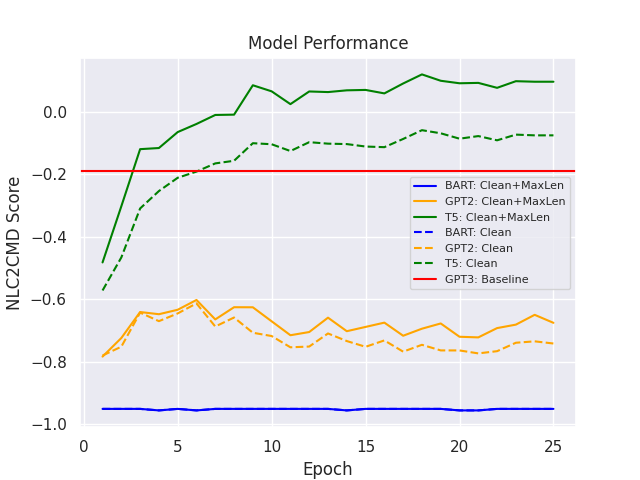
\includegraphics[scale=0.6]{metric.png}
\end{center}
Despite improving on the training objective, all 3 of these models still
produced garbled and verbose responses. Repetition was common for all 3,
although most with BART. GPT-2 had a tendency to ``ramble;'' it was not uncommon
for GPT-2 to generate natural language intermixed with bash commands. It also
frequently produced multiple ``target stories.'' Here we define a target story
as a section of output text that begins with the special token
\texttt{<|target|>}, which was used to denote the beginning of a bash command
in the encoded input. Here is an example row of output from the modeling process with GPT-2:
\begin{minted}{json}
{
  "source": "List the files from the current directory tree that contain
    lines matching regular expression '^From:.*unique sender',
    ignoring ~/src and ~/bin",
  "target": "find Path -name Regex -prune -or -name Regex -prune \
    -or -type f -print | xargs -I {} grep -E -i -l Regex {}",
  "prediction": "<|endoftext|> <|source|> List the files from the current
    directory tree that contain lines matching regular expression
    '^From:.*unique sender', ignoring ~/src and ~/bin <|target|><|endoftext|>
    <|endoftext|><|endoftext|><|endoftext|><|endoftext|><|endoftext|>
    The first day of the year is a long one for the first day of the year.
    <|target|> find Path -name Regex -daystart -type f -print0 \
    | xargs -0 -I {} grep -H Regex {}   "
},
\end{minted}
Here you can see several types of errors affecting performance. A detailed
analysis is left for the subsequent section, but here we will highlight 3
issues that motivated our postprocessing. First, you can see that GPT-2 outputs
multiple target stories, i.e. in the prediction, there are two chunks of text
following a special target token. Second, we can see that GPT-2 still had
internalized the meaning of the target token, because it continued to predict
natural language as well as special end of sentence tokens,
\texttt{<|endoftext|>}, after the target token. Third, we can see hints of
GPT-2's pretraining through the inserted sentence ``The first day of the year is
a long one for the first day of the year.'' This suggests that GPT-2 is still
heavily biased toward its pretraining data, despite being fine-tuned to produce
bash commands. BART and T5 had similar errors, but those are also left for
analysis.
\par
Many competitors in the NLC2CMD competition actually crafted extremely
sophisticated postprocessing techniques. Some used ensemble models, other
implemented a custom structured beam-search. Given the time limitations for
this project, we elected for a rule-based approach. We ran simple functions
that could be composed across model predictions. We would then score the
prediction after postprocessing. We designed 3 postprocessing functions to
address our main problems: (1) multiple target texts, (2) repetition or
rambling, and (3) binary prediction.
\par
Looking at the predictions, we noticed that, most often, the target text
closest to a bash command was the last sequence GPT-2 generated. Accordingly, we
wrote a function we named \texttt{clean} that selected the last chunk of text
associated with a target command. Second, because the scoring metric penalizes
incorrect or excessive flags, we tried to trim repetitions and rambling with a
function called \texttt{max\_len}. Tokenizing by separating on whitespace, we
collapsed repeated tokens and limited the maximum number of tokens to 15.
Lastly, we attempted to do binary matching. Because the entire prediction's
score hinges largely on selecting the right binary, we wrote a function that
attempted to find the first token in a sequence that closely matched a top 100
bash utility name. This last function did not improve performance much, and so
was dropped when evaluating our final models. Using the above prediction and
running through \texttt{clean} yields the following:
\begin{verbatim}
find Path -name Regex -daystart -type f -print0 | xargs -0 -I {} grep -H Regex {}
\end{verbatim}
And then through \texttt{max\_len}:
\begin{verbatim}
find Path -name Regex -daystart -type f -print0 | xargs -0 -I {} grep -H
\end{verbatim}
While these cleaning techniques are quite crude, they significantly improve
scores. The best model scores under different preprocessing functions along
with the GPT3 baseline are recorded in the following table:

\begin{center}
	\begin{tabular}{rcccc}
		\toprule
		model & raw   & clean & clean+max\_len \\
		\midrule
		GPT-2  & -0.95 & -0.61 & -0.60          \\
		BART  & -0.95 & -0.95 & -0.95          \\
		T5    & -0.13 & -0.06 & \textbf{0.12}  \\
		% GPT-2  & -0.951691 & -0.613975 & -0.602972      \\
		% BART  & -0.951691 & -0.951691 & -0.951691      \\
		% T5    & -0.125204 & -0.059434 & 0.119156       \\
		\hline
		GPT3  & -0.19 & -0.19 & -0.19          \\
		\bottomrule
	\end{tabular}
\end{center}

\section{Analysis}
The first task in analyzing model performance was error analysis. We checked all predictions on the test set by epoch for each model to discover generalizations, which are summarized in the following table:
\newcolumntype{L}{>{\centering\arraybackslash}m{3.7cm}}
\newcolumntype{M}{>{\centering\arraybackslash}m{1.7cm}}
\newcolumntype{N}{>{\centering\arraybackslash}m{8.5cm}}
\newcolumntype{O}{>{\centering\arraybackslash}m{6cm}}

\begin{center}
	\begin{tabular}{ |M|L|L|L| }
		\hline
		\textbf{Model}                                         & \textbf{BART}                                              & \textbf{T5} & \textbf{GPT-2} \\
		\hline
		Primary sources of error                               &
		missing or invalid binaries (like "findfind")          &
		repetition of sequences or redundant tokens            &
		wrong interpretations of the invocation                                                                                                            \\
		\hline
		Example target                                         & find Path -name Regex -print | xargs -l -i -I {} wc {} {}, &
		yes Regex | sed Program                                &
		sort <( sort -u File ) File File | uniq -u                                                                                                         \\
		\hline
		Example prediction                                     &
		Path -name Regex |print0 wargs -I QuantityI -I {} wc - & yes Regex | headt Program yes yes yes yes yes yes          &
		find Path -iname Regex -exec grep -i Regex {}                                                                                                      \\
		\hline
	\end{tabular}
\end{center}

Because both BART nor GPT-2 struggled to correctly capture the target binaries,
they received significant scoring penalties. The redundant binaries or flags
and arguments, on the other hand, were not so harshly penalized; consequently,
T5 was able to edge out the GPT-3 baseline. Curiously, the BART model tended to
get the wrong starting binary for almost all the examples, but did very well in predicting the remainder of the command. Here are some examples of this pathology:
\begin{center}
	\begin{tabular}{ |O|O| }
		\hline
		\textbf{Target}      & \textbf{Prediction} \\
		\hline
		comm -2 -3 File File &
		-2 -3 File File                            \\
		\hline
		chown Regex -R File  &
		own Regex -R File                          \\
		\hline
		mv -f File File      & mmv -f File File    \\
		\hline
	\end{tabular}
\end{center}
Investigating this further, we first confirmed that the model was improving over epochs.
We analyzed a single invocation: ``display all the html files in the current
folder excluding search in the path ./foo'' over several epochs. Although none
of the predictions correctly captured the target binary ``find,'' the model did
improve in pruning trailing repetitions.
\begin{center}
	\begin{tabular}{|M|N|}
		\hline
		Target                 & find Path -path Regex -prune -or -type f -name Regex                                                             \\
		\hline
		Prediction (1 epoch)   & findfind Path -name Regex -prune -or -name f -name Regexexecexecexecexecexecexecexecexecexecexecexecexecexecexec \\
		\hline
		Prediction (6 epochs)  & Path -path Regex -prune -or -path f -name Regex -findfindfindfind                                                \\
		\hline
		Prediction (14 epochs) & findfind Path -path Regex -prune -or -name f -name Regex -print - -                                              \\
		\hline
	\end{tabular}
\end{center}
One possible reason for this aberrant behavior is that BART, while doing a reasonable job in capturing the intent of the sentence, struggled to develop individual token accuracy; in particular, the accuracy of the binary token. Predicting a binary given only the natural language and the beginning of sentence special token was difficult. Because predicting the binary is so important, we hypothesize that separating BART training into the following to phases may improve performance: (1) train only on the natural language command and the singular token corresponding to the correct Bash utility, and then (2) fine-tune the model further with the full, templated Bash commands. Improving binary prediction in BART would likely make it competitive with T5.
\par
We also investigated GPT-2 prediction errors. Here is an example prediction for the natural language invocation: ``Change the ownership of all files in the current directory tree from root to www-data'':

\begin{verbatim}
<|endoftext|> <|source|> Change the ownership of all files in the current 
directory tree from root to www-data <|target|> (omit 23 <|endoftext|> tokens 
here) Synchronize file systems to /tmp/ and output the result to console 
<|target|> df File | awk Program | xargs -I {} ls -a -l -d -S -r File
\end{verbatim}
The model incorrectly generated another invocation: ``Synchronize file systems to /tmp/ and output the result to console.'' This has greater implications than simply generating additional cruft to be trimmed; it actually corrupts the hidden state of the model. Consequently, the final prediction was orthogonal to the target command \texttt{find Path -user Regex -exec chown Regex \{\}}.
\par
The last error class, which was demonstrated by all 3 models was ``rambling,'' or inserting additional command sequences after the target sequence. Here is an example:
\begin{verbatim}
target    : cat File | sort -r -h 
prediction: cat File | sort -n -r | grep -v Regex
\end{verbatim}
This suggests that all the models failed to generate the end of text token in the correct location.
\par
While all of these models could be improved with longer training, phased training, and more sophisticated post-processing, the principal factor affecting performance was data size. 10,000 examples is insufficient to generate very accurate translations, and we were unable to find additional data sources that did not require significant preprocessing.


\section{Conclusion}
The three main discoveries of this project were: (1) the size of the dataset is
the most important factor in performance, (2) postprocessing is required,
especially when training on limited data, and (3) signaling structure to your
model is difficult and subtle but dramatically affects performance, as seen
with BART. While we are satisfied to have surpassed the GPT-3 baseline, the
competition winner achieved a score of 0.53, which still significantly exceeds
the 0.12 achieved by our T5 model. This team, however, augmented their data by
scraping Stack Overflow and similar website. They also implemented a variety of
additional techniques, which included a custom beam search and ensemble
classification, which were out of the scope of this project. We believe that
success on this task likes principally in cultivating a larger dataset of
parallel translations. T5 was able to achieve notable performance using only
10,000 examples. With 100,000, we are confident that T5 may well exceed the
performance of the top model, even in the absence more sophisticated
techniques.


\bibliographystyle{unsrt}
\bibliography{references}

\end{document}
